% class
\documentclass[a4paper,12pt,xelatex,ja=standard]{bxjsarticle}

% packages
%% mathematical notations
\usepackage{amsthm,amsmath,amssymb,amsfonts} % mathematical notations
\usepackage{bm} % bold character
\usepackage{latexsym} % more mathematical notations
\usepackage{physics} % physical notations
%% graphs
\usepackage{graphicx, xcolor} % graph
\usepackage{circuitikz} % for circuit elements
\usepackage{float} % positioning of graphs
\usepackage{siunitx} % SI units
\usepackage{tikz} % graphic elements
\usepackage{wrapfig} % must be after float package.
%% type system
\usepackage{bussproofs} % proof tree
%% code
\usepackage[ruled,vlined]{algorithm2e} % pseudo code
\usepackage{listings} % source code
\usepackage{inconsolata}
\lstset{
  basicstyle=\footnotesize,
  numbers=left,
  frame=single
}

% Basic information
\title{電子情報学専攻 \, 専門 \\ 平成24年 \, 解答・解説}
\author{diohabara}
\date{\today}

\begin{document}
\maketitle

\section*{第1問\ 電気・電子回路}

\section*{第2問\ 論理回路}
\subsection*{(1)}
順序回路とは過去の入力によって決まる状態と現在の入力によって出力が決まる回路である。

\subsection*{(2)}

JKフリップフロップの特性表は以下の通りである。

\begin{table}[H]
  \begin{tabular}{|l|l|l|}
  \hline
  J & K & Q                  \\ \hline \hline
  0 & 0 & Q (hold)           \\ \hline
  0 & 1 & 0 (reset)          \\ \hline
  1 & 0 & 1 (set)            \\ \hline
  1 & 1 & $\bar{Q}$ (toggle) \\ \hline
  * & * & Q (hold)           \\ \hline
  \end{tabular}
\end{table}

また、8進カウンタの動作は以下の表の通りになる。

\begin{table}[H]
  \centering
  \begin{tabular}{|l|l|l|l|l|l|l|}
  \hline
  $n$ & $Q^n_2$ & $Q^n_1$ & $Q^n_0$ & $Q^n_2 \to Q^{n+1}_2$ & $Q^n_1 \to Q^{n+1}_1$ & $Q^n_0 \to Q^{n+1}_0$ \\ \hline \hline
  0 & 0 & 0 & 0 & $0 \to 0$ (hold)   & $0 \to 0$ (hold)   & $0 \to 1$ (toggle) \\ \hline
  1 & 0 & 0 & 1 & $0 \to 0$ (hold)   & $0 \to 1$ (toggle) & $1 \to 0$ (toggle) \\ \hline
  2 & 0 & 1 & 0 & $0 \to 0$ (hold)   & $1 \to 1$ (hold)   & $0 \to 1$ (toggle) \\ \hline
  3 & 0 & 1 & 1 & $0 \to 1$ (toggle) & $1 \to 0$ (toggle) & $1 \to 0$ (toggle) \\ \hline
  4 & 1 & 0 & 0 & $1 \to 1$ (hold)   & $0 \to 0$ (hold)   & $0 \to 1$ (toggle) \\ \hline
  5 & 1 & 0 & 1 & $1 \to 1$ (hold)   & $0 \to 1$ (toggle) & $1 \to 0$ (toggle) \\ \hline
  6 & 1 & 1 & 0 & $1 \to 1$ (hold)   & $1 \to 1$ (hold)   & $0 \to 1$ (toggle) \\ \hline
  7 & 1 & 1 & 1 & $1 \to 0$ (toggle) & $1 \to 0$ (toggle) & $1 \to 0$ (toggle) \\ \hline
  8 & 0 & 0 & 0 & $0 \to 0$ (hold)   & $0 \to 0$ (hold)   & $0 \to 1$ (toggle) \\ \hline
  \end{tabular}
\end{table}

表のtoggleとなっている際の$Q_0, Q_1, Q_2$に注目して、以下の式が成り立つ。

\begin{equation*}
  \centering
  \begin{split}
    &J_0 = K_0 = 1 \\
    &J_1 = K_1 = Q_0 \\
    &J_2 = K_2 = Q_1 Q_0
  \end{split}
\end{equation*}

以上より求める8進カウンタの回路は以下の通り。

\begin{figure}[H]
  \centering
  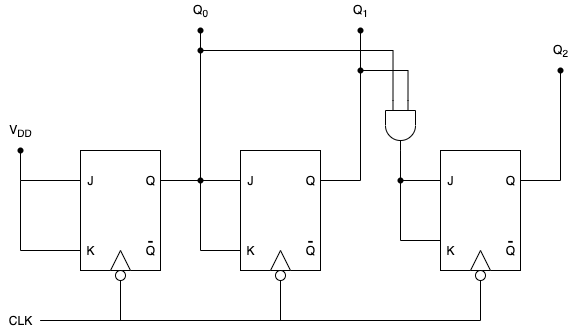
\includegraphics[width=11cm]{images/8_counter.png}
\end{figure}

\subsection*{(3)}

求める同期式5進カウンタの動作表は次の通り。

\begin{table}[H]
  \centering
  \begin{tabular}{|l|l|l|l|l|l|l|}
  \hline
  $n$ & $Q^n_2$ & $Q^n_1$ & $Q^n_0$ & $Q^n_2 \to Q^{n+1}_2$ & $Q^n_1 \to Q^{n+1}_1$ & $Q^n_0 \to Q^{n+1}_0$ \\ \hline \hline
  0 & 0 & 0 & 0 & $0 \to 0$ (hold)   & $0 \to 0$ (hold)   & $0 \to 1$ (toggle) \\ \hline
  1 & 0 & 0 & 1 & $0 \to 0$ (hold)   & $0 \to 1$ (toggle) & $1 \to 0$ (toggle) \\ \hline
  2 & 0 & 1 & 0 & $0 \to 0$ (hold)   & $1 \to 1$ (hold)   & $0 \to 1$ (toggle) \\ \hline
  3 & 0 & 1 & 1 & $0 \to 1$ (toggle) & $1 \to 0$ (toggle) & $1 \to 0$ (toggle) \\ \hline
  4 & 1 & 0 & 0 & $1 \to 0$ (toggle) & $0 \to 0$ (hold)   & $0 \to 0$ (hold)   \\ \hline
  5 & 0 & 0 & 0 & $0 \to 0$ (hold)   & $0 \to 0$ (hold)   & $0 \to 1$ (toggle) \\ \hline
  \end{tabular}
\end{table}

表のtoggleとなっている際の$Q_0, Q_1, Q_2$に注目して、以下の式が成り立つ。

\begin{equation*}
  \begin{split}
    &J_0 = K_0 = \bar{Q}_2 \\
    &J_1 = K_1 = Q_0 \\
    &J_2 = Q_1 Q_0 \\
    &K_2 = \bar{Q}_2
  \end{split}
\end{equation*}

以上より求める5進カウンタの回路は以下の通り。

\begin{figure}[H]
  \centering
  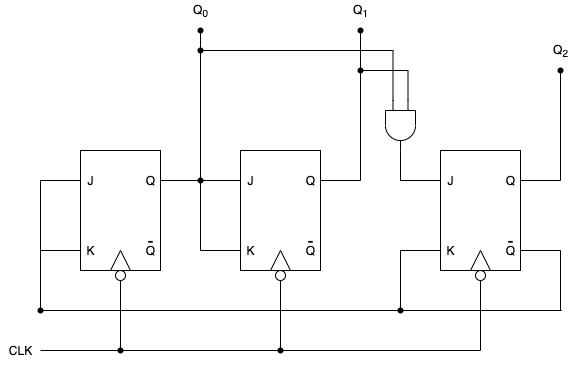
\includegraphics[width=11cm]{images/5_counter.png}
\end{figure}

\subsection*{(4)}
本題の回路の動作表は以下の通り。
\begin{table}[H]
  \begin{tabular}{|l|l|l|l|l|l|l|}
  \hline
  $n$ & $Q^n_2$ & $Q^n_1$ & $Q^n_0$ & $Q^n_2 \to Q^{n+1}_2$ & $Q^n_1 \to Q^{n+1}_1$ & $Q^n_0 \to Q^{n+1}_0$ \\ \hline \hline
  0 & 1 & 1 & 0 & $1 \to 0$ (toggle) & $1 \to 0$ (toggle) & $0 \to 1$ (toggle) \\ \hline
  1 & 0 & 0 & 1 & $0 \to 0$ (hold)   & $0 \to 0$ (hold)   & $1 \to 0$ (toggle) \\ \hline
  2 & 0 & 0 & 0 & $0 \to 0$ (hold)   & $0 \to 1$ (toggle) & $0 \to 0$ (hold)   \\ \hline
  3 & 0 & 1 & 0 & $0 \to 1$ (toggle) & $1 \to 0$ (toggle) & $0 \to 1$ (toggle) \\ \hline
  4 & 1 & 0 & 1 & $1 \to 1$ (hold)   & $0 \to 1$ (toggle) & $1 \to 0$ (toggle) \\ \hline
  5 & 1 & 1 & 0 & $1 \to 0$ (toggle) & $1 \to 0$ (toggle) & $0 \to 1$ (toggle) \\ \hline
  \end{tabular}
\end{table}

表のtoggleとなっている際の$Q_0, Q_1, Q_2$に注目して、以下の式が成り立つ。

\begin{equation*}
  \begin{split}
    &J_0 = K_0 = Q_0 \bar{Q}_1 + \bar{Q}_0 Q_1 \\
    &J_1 = K_1 = \bar{Q}_0 + \bar{Q}_1 Q_2 \\
    &J_2 = Q_1 \\
    &K_2 = \bar{Q}_0 \\
  \end{split}
\end{equation*}

以上より求める本題の回路は次の通り。

\begin{figure}[H]
  \centering
  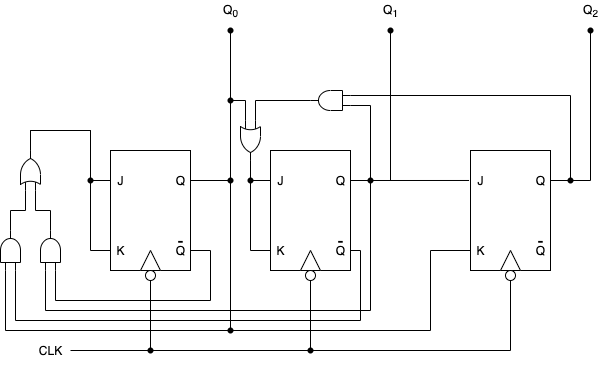
\includegraphics[width=11cm]{images/2013_counter.png}
\end{figure}

\section*{第3問\ アルゴリズム}
\subsection*{(1)}

\subsection*{(2)}

\subsection*{(3)}

\subsection*{(4)}

\subsection*{(5)}

\section*{第4問\ ネットワーク}

\section*{第5問\ 情報理論}
\subsection*{(1)}

\subsection*{(2)}

\subsection*{(3)}

\subsection*{(4)}

\subsection*{(5)}

\end{document}

